\documentclass{article}
\usepackage{preamble}

\title{Thesis Preparation Report}
\author{Jonas Tonny Nielsen \and Jonas Lomholdt}
\date{\today}

\begin{document}

\maketitle

\listoftodos

\tableofcontents
\listoffigures
%\listoftables

\todo{Hand-in Jan 8th}

\section{Introduction} % Introduction to the project
A number of studies have shown that introducing clicker systems, also known as Classroom Response Systems (CRS),  into classrooms has a positive effect on learning outcomes and classroom interactivity \cite{yourstone2008classroom, siau2006use, lantz2014effectiveness}. 

The idea of a CRS is not a new one and low-tech versions have been used in classrooms before, where students simply hold up a piece of paper, called a response card, with their answers \cite{ralph1994effects}. 
Later more modern versions are introduced, the so called \emph{clickers}. A clicker is a device, that allows users (and in many cases, students) to respond to questions in a classroom environment. These systems are defined by \citeA{lantz2014effectiveness} in it's most common form as 

\begin{quote}
    \emph{"[...] individual response devices held by individual students allowing them to quickly and anonymously respond to multiple choice questions presented in class. A receiver attached to a classroom computer collects and summarizes the responses instantly and projects them graphically onto the screen for students and the educator to see"} \cite{lantz2014effectiveness}
\end{quote}

As described above, the clicker itself is used for collecting answers from the students via a clicker device. Many different versions exists, and one example can be seen in figure \ref{fig:iclicker} below. The device connects to a receiver in the classroom and the receiver is then again connected to a computer that stores and displays the data through a piece of software. 

\begin{figure}[H]
\capstart
	\centering
		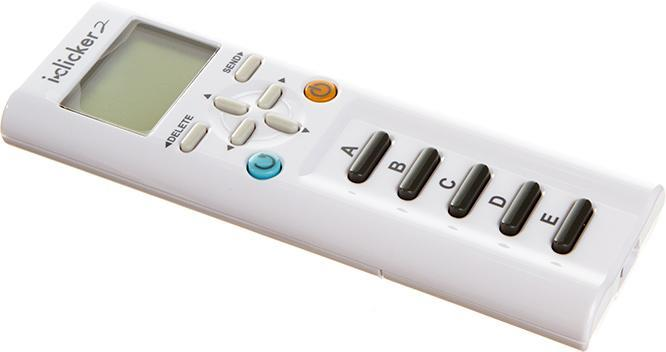
\includegraphics[width=\textwidth]{iclicker.jpg}
        %\missingfigure{iClicker - An example of an iClicker}
	\caption[iClicker2]{One example of a clicker device called the iClicker2 \label{fig:iclicker}}
\end{figure}


%%% explain a poll, and 'polling' and 'polling devices'
%%% explain polling fatigue


%\cite{yourstone2008classroom}
%\maskciteyear{einstein}. 

\section{Literature Review} % What is already known and done + existing solutions?
Many different classroom response system solutions already exists, and all seem to have a different approach. Some are made exclusively for children or ground-schoolers (\url{https://kahoot.it}), and some are feature rich, made for conferences and classrooms (\url{http://socrative.com}, \url{https://www.polleverywhere.com} and \url{https://www.iclicker.com/} etc.). The most appealing and well implemented version we could find was Mentimeter (\url{https://www.mentimeter.com}), which supports many of the features that would be expected of a fully functional CRS. Most of the existing literature is centered around physical clickers and the learning outcomes of using them, though there seems to be a lack of research of the use of such systems within the last few years, where smartphones has become widespread and popular among students \cite[p.~329]{stowell2015use}.


Some of the least resent literature dating back to around 2007, is mainly focused on physical clicker devices, where the students buy actual "remote controls" for polling, in a time where more modern solutions (including the smartphone) has not yet matured. And even today, the physical clicker devices still seem to play a significant role in the "clicker community". \citeA{stowell2015use} explains how the use of clicker systems on physical devices has a greater response rate compared to mobile, but with no significant differences in the final grades. Also the introduction of students bringing their own devices (the so called \emph{Bring Your Own Device}) introduces new issues such as internet connectivity and the risk of being distracted by the device itself (pp. 331-332).


One of the main reasons to use a CRS is the importance of interactivity in learning \cite{draper2004increasing}. Studies find that CRS engages interactivity, helps students stay active during lectures \cite[p.~116]{moredich2007engaging} and improves learning \cite<e.g.,>{siau2006use, yourstone2008classroom}. While \citeA{yourstone2008classroom} focuses on actual results in learning outcomes, then most other studies take on a qualitative approach and evaluate teachers and students by asking to their engagement, participation and learning outcomes \cite<e.g.,>{moredich2007engaging}. The latter approach seems to be the most widespread in the literature and focuses more on whether or not students feel an increased engagement and participation rather than their actual performance and examination results. 

\citeA{stowell2007benefits} takes on the qualitative approach where they ask into students emotions towards an introductory psychology class before, during and after lecture. The study compares standard lectures to hand raising, response card and "clicker" lectures\footnote{Standard lectures are thought of as normal lectures where the teacher asks open ended questions to the students. Hand raising is the approach where students are asked to raise their hand if they agree to a statement. Response cards are cards labeled 1, 2, 3, 4 or A, B, C, D and are sort of the same as hand raising \cite[p.~254]{stowell2007benefits}.}. They find that more correct answers to questions are present in response card lectures but explains the much higher correctness with the ability to see what peers are answering \cite[p.~257]{stowell2007benefits}. The same applies for hand raising. Furthermore the study finds that there's no huge impact on emotions towards the class depending on which kind of lecture is taught (i.e. standard, hand raising, response card and "clicker") \cite{stowell2007benefits}.




Among the biggest studies of CRS is \emph{Increasing interactivity in lectures using an electronic voting system} by \citeA{draper2004increasing}. This particular study took place over a two year period and found (among other things) that the benefits increases as teachers became aware how to exploit the pedagogy behind the system \cite[p.~93]{draper2004increasing}. The study took place in a time where there was a need for physical hardware (e.g., remote controllers and receivers) in order to facilitate a CRS. This study addresses the need to learn how to proper use a CRS in order to get the benefits from it. This a whole separate field of study, and to name a few \todo{name a few}



\section{Method}


\section{Implementation - Our Contribution - how we are improving this}
Our idea is to implement a classroom response system from scratch. The system should include features that support asking and answering technical questions. 
%%% We should be able to display code, including linenumbers and syntax highlighting!


\subsection{Possible implementation thoughts}

\subsection{Features} % The features of the system

%Users
    %user roles
        %Admin
        %Teacher
        %Student
    %Profile picture
%Classrooms
    %Search for classrooms
    %Create classroom (teachers only)
    %Invite students to classrooms
    %Group questions by tags
    %Invite to classroom by email
    %Request access to classroom
    %Delete classrooms
%Questions
    %Create questions of different types (teachers only)
        %Multiple Choice questions
        %Include pictures
        %Fill-in-the-blank questions
    %Questions should be open and closeable by teachers (students can/cannot answer)
    %Students should be notified when new questions are available
    %Questions should be publishable
    %Delete questions
    %Add tags/labels
%Dashboard (teacher)
    %Graphs with answer overview
    %Real-time feed of answers (Pusher/Sockets, green check mark if answered red cross if not-ish)
%Dashboard (student)
    %See classrooms
    %See question history


% RESTfull service 
% thesis.com/classroom/advanced-programming-2015/question/16/

\subsection{Database design}


\begin{figure}[H]
\capstart
	\centering
		%\includegraphics[scale=0.65]{ClassHTMLList.png}
        \missingfigure{Database Design}
	\caption{Database Design\label{fig:database-design}}
\end{figure}






%--------------------REFERENCES--------------------%
\bibliographystyle{apacite}
\bibliography{ref.bib}


\end{document}
